\documentclass[10pt,journal,compsoc]{IEEEtran}
% * <carlos.segarra@bsc.es> 2017-09-21T09:08:41.072Z:
%
% ^.

\ifCLASSOPTIONcompsoc
  % IEEE Computer Society needs nocompress option
  % requires cite.sty v4.0 or later (November 2003)
  \usepackage[nocompress]{cite}
\else
  % normal IEEE
  \usepackage{cite}
\fi
\usepackage[pdftex]{graphicx}
\usepackage{amsmath}
\newtheorem{definition}{Definition}
\interdisplaylinepenalty=2500
%\usepackage{algorithmic}
\usepackage{array}
\ifCLASSOPTIONcompsoc 			     	 \usepackage[caption=false,font=footnotesize,labelfont=sf,textfont=sf]{subfig}
\else
  \usepackage[caption=false,font=footnotesize]{subfig}
\fi
\ifCLASSOPTIONcaptionsoff
  \usepackage[nomarkers]{endfloat}
 \let\MYoriglatexcaption\caption
 \renewcommand{\caption}[2][\relax]{\MYoriglatexcaption[#2]{#2}}
\fi
\usepackage{url}
\hyphenation{op-tical net-works semi-conduc-tor}

\usepackage{algorithm}% http://ctan.org/pkg/algorithms
\usepackage{algpseudocode}% http://ctan.org/pkg/algorithmicx

%URL
\usepackage{hyperref}
\usepackage{tabularx}

%Plotting
\usepackage{tikz}
%\usepackage{tikz-3dplot} 
\usepackage{pgfplots}

\usepackage{varwidth}% http://ctan.org/pkg/varwidth

%Code snippets
\usepackage{xcolor}
\usepackage{listings}
\definecolor{codegreen}{rgb}{0,0.6,0}
\definecolor{codegray}{rgb}{0.5,0.5,0.5}
\definecolor{codepurple}{rgb}{0.58,0,0.82}
\definecolor{backcolour}{rgb}{0.98,0.98,0.95}
\lstdefinestyle{mystyle}{
    backgroundcolor=\color{backcolour},   
    commentstyle=\color{codegreen},
    keywordstyle=\color{magenta},
    numberstyle=\tiny\color{codegray},
    stringstyle=\color{codepurple},
    basicstyle=\footnotesize\ttfamily,breaklines=true,
    breakatwhitespace=false, 
    xleftmargin=20pt, 
    xrightmargin=20pt,       
    breaklines=true,                 
    captionpos=b,                    
    keepspaces=true,                 
    numbers=left,                    
    numbersep=5pt,                  
    showspaces=false,                
    showstringspaces=false,
    showtabs=false,                  
    tabsize=2,
    framextopmargin=50pt,
    frame=bottomline,
    basicstyle=\footnotesize\ttfamily,
    language=Python
}
\lstset{literate=
  {á}{{\'a}}1 {é}{{\'e}}1 {í}{{\'i}}1 {ó}{{\'o}}1 {ú}{{\'u}}1
  {Á}{{\'A}}1 {É}{{\'E}}1 {Í}{{\'I}}1 {Ó}{{\'O}}1 {Ú}{{\'U}}1
  {à}{{\`a}}1 {è}{{\`e}}1 {ì}{{\`i}}1 {ò}{{\`o}}1 {ù}{{\`u}}1
  {À}{{\`A}}1 {È}{{\'E}}1 {Ì}{{\`I}}1 {Ò}{{\`O}}1 {Ù}{{\`U}}1
  {ä}{{\"a}}1 {ë}{{\"e}}1 {ï}{{\"i}}1 {ö}{{\"o}}1 {ü}{{\"u}}1
  {Ä}{{\"A}}1 {Ë}{{\"E}}1 {Ï}{{\"I}}1 {Ö}{{\"O}}1 {Ü}{{\"U}}1
  {â}{{\^a}}1 {ê}{{\^e}}1 {î}{{\^i}}1 {ô}{{\^o}}1 {û}{{\^u}}1
  {Â}{{\^A}}1 {Ê}{{\^E}}1 {Î}{{\^I}}1 {Ô}{{\^O}}1 {Û}{{\^U}}1
  {œ}{{\oe}}1 {Œ}{{\OE}}1 {æ}{{\ae}}1 {Æ}{{\AE}}1 {ß}{{\ss}}1
  {ű}{{\H{u}}}1 {Ű}{{\H{U}}}1 {ő}{{\H{o}}}1 {Ő}{{\H{O}}}1
  {ç}{{\c c}}1 {Ç}{{\c C}}1 {ø}{{\o}}1 {å}{{\r a}}1 {Å}{{\r A}}1
  {€}{{\euro}}1 {£}{{\pounds}}1 {«}{{\guillemotleft}}1
  {»}{{\guillemotright}}1 {ñ}{{\~n}}1 {Ñ}{{\~N}}1 {¿}{{?`}}1
}
\lstset{style=mystyle}
%\pgfplotsset{compat=1.14}

\begin{document}

\title{DBSCAN for PyCOMPS\\ \LARGE{A distributed approach}}

\author{Carlos~Segarra \\ 
\href{mailto:carlos.segarra@bsc.es}{carlos.segarra@bsc.es}}

\IEEEtitleabstractindextext{%
\begin{abstract}
% Abstract structure:
% - Introduce the importance of the topic and the scope. DONE
% - Describe very briefly what has been done (general description without details). DONE
% - Give a global overview of the achievements. DONE
% - REVIEW: 

The DBSCAN algorithm is one of the most popular clustering techniques used nowadays. However there is a lack of distributed implementations. Additionally, parallel implementations fail when they try to scale to hundreds of cores. The scope of this report is to provide a novel implementation of the algorithm that behaves well in large distributed architectures and with big datasets. Using the PyCOMPSs framework and testing on the Mare Nostrum 4 supercomputer, encouraging results have been obtained reaching a 2467 speedup when run with 4096 cores. Everything whilst keeping the code clean and transparent to the user.
\end{abstract}

\begin{IEEEkeywords}
DBSCAN, Clustering, Machine Learning, Distributed Computing, COMPSs, PyCOMPSs
\end{IEEEkeywords}}
\maketitle
\IEEEdisplaynontitleabstractindextext
\IEEEpeerreviewmaketitle

\IEEEraisesectionheading{\section{Introduction}\label{sec:introduction}}

% Introduction structure {
% - Introduce the topic and the scope (give a use case can be helpful). DONE
% - Brief overview of DBSCAN (what is it used for?) DONE
% - Purpose of the article. * DONE
% - Motivation and objective/s. * ??
% - Contribution of the paper. * DONE
% - Define the structure of the article DONE
%   * These points can be in another order.

Big data and data mining is on the daily agenda of nowadays' engineers and having tools to process and analyze this data quickly is of vital importance. Precisely, machine learning, and more precisely, unsupervised learning and clustering are useful for detecting trends and patterns between data without needing the user to previously classify it. The DBSCAN belongs to this family of methods and is useful for detecting non-convex (arbitrarily-shaped) clusters as explained in Section \ref{sec:background}.

This document covers the first implementation of the DBSCAN clustering algorithm within the COMPSs \cite{compss} framework for distributed computing. The main scope of this paper is to accomplish a reasonable speedup when scaling to thousands of cores, being able to process datasets of hundreds of thousands or millions of points in a reasonable amount of time.

Our main contribution is a simple algorithm, completely sequential at first glance, that a standard programmer without much knowledge on concurrency could maintain and develop, programmed in Python (which enhances even more the readability) that scales to thousands of nodes and performs well on big clusters. 

The structure of the paper is the following. Section \ref{sec:related_work} covers related work, other attempts to implementing a parallel version of the DBSCAN in other programming frameworks as well as other clustering algorithms. It briefly covers different benchmarks related to performance and emphasizes the novelty of our proposal. Following along, Section \ref{sec:background} introduces the state of the art of clustering algorithms, describes the Density-Based Spatial Clustering Algorithm the programming model chosen for the implementation and covers the environment where tests have been performed. Section \ref{sec:implementation} describes the algorithm developed to fulfill the scope of the paper, the dependency graph drawn by it and covers possible equivalence issues faced when reinterpreting a sequential algorithm as a parallel one. Section \ref{sec:performance} summarizes all the tests performed with synthetic and real data, presents the results and gives a critical review to the algorithm using post-mortem analysis tools and tracing. Lastly Section \ref{sec:conclusion} gathers the conclusions obtained and proposes further developments that did not fit our initial scope.
% }

\section{Related Work} \label{sec:related_work}

Quickly after the algorithm was first presented (1996) the necessity to feed the clustering algorithm with big datasets arose. First approaches of DBSCAN parallelization only dealt with the region query issue which is indeed where more calculus power is invested. For instance, \cite{related_1} presents a skeleton-structured program where slaves are responsible for answering the regions query performed by the master.

Latter developments started including smart data partitioning. \cite{related_2} proposes what has become a standard procedure for distributed implementations of the DBSCAN. Initially data is efficiently divided, secondly a series of partial clusterings are performed and final results are merged by the master. Most implementations differ on both the partition and the merging. \cite{related_2} divides data using a low-precision hierarchical clustering algorithm and merges the data using a graph connectivity technique similar to the one used in this paper. Graph connectivity techniques are also used in \cite{related_4}. Yaobin HE et. al \cite{related_3} propose a novel partitioning method based on computational costs predictions and merge results using a 4 step MapReduce strategy. 

Latest developments focus on flexibility and scalability to high feature datasets. A. Lulli \cite{related_5} presents a Spark-based algorithm that does not require euclidean metric and that works with arbitrary data.

The novelty of our proposal lies that in all the previously mentioned papers, the code might be quite difficult to understand and specially to mantain for a user. Taking advantage of the COMPSs framework for distributed programming, the final code produced is highly-readable.
% Add related works (publications) with the same or similar objective (even for another clustering algorithms or frameworks). DONE

% Don't forget to point out the differences between other proposals and the one presented in the paper. DONE 
% I would try to concentrate the main difference/novelty as the last phrase of this section to remark what makes this work innovative compared to others. DONE




%%%%%%%%%%%%%%%%%%%%%%%%%%%%%%%%%%%%%%%%%%%%%%%%%%%%%%%%%%%%
%%%%%%%%%%%%%%%%%%     BACKGROUND       %%%%%%%%%%%%%%%%%%%%
%%%%%%%%%%%%%%%%%%%%%%%%%%%%%%%%%%%%%%%%%%%%%%%%%%%%%%%%%%%%


\section{Background} \label{sec:background}

% JC: This section can be used to provide the necessary background for understanding the following sections.
% JC: Here, DBSCAN can be defined formally, as well as PyCOMPSs.

This section provides the necessary information to firstly understand the implementation proposed and secondly to contextualize the tests performed.

\subsection{The algorithm: DBSCAN} \label{the_algorithm}

% Formal definition of DBSCAN

The \textbf{D}ensity-\textbf{B}ased \textbf{S}patial \textbf{C}lustering \textbf{A}lgorithm with \textbf{N}oise (\textbf{DBSCAN}) is a clustering algorithm based on point density. It was proposed in 1996 \cite{ReferencePaper} and has become one of the reference techniques for non-supervised learning. To take a first dive into the implementation, a few previous definitions are mandatory.

\begin{definition}
The $\varepsilon$\textbf{-neighborhood} of a point $p$ from a dataset $D$ and given a distance $d$ is
$$N_{\varepsilon}(p) = \lbrace q \in D: d(p,q) < \varepsilon \rbrace$$ 
\end{definition}

The general approach partitions the set of points in three subsets:
\begin{definition}
\begin{itemize}
\item A point $p$ is said to be \textbf{\textit{core point}} if it has over \textit{minPoints} neighbors within its $\varepsilon$-neighborhood.
\item A point $p$ is said to be \textbf{\textit{reachable}} if it lies within a $\varepsilon$-neighborhood of a core point in spite of not being one.
\item A point $p$ is said to be \textbf{\textit{noise}} if it does not fulfil any of the previous definitions.
\end{itemize}
\end{definition}

\begin{definition}
A \textbf{Cluster} $C$ is a subset of a dataset $D$ such that for all $p \in C$:
\begin{itemize}
\item[(i)] $p$ is a core-point or reachable
\item[(ii)] $\forall p,q \in C, \exists p_1, \ldots,  p_r$ fulfilling (i) such that $p \in N_{\varepsilon}(p_1)$, $p_i \in N_{\varepsilon}(p_{i+1})$ and $p_r \in N_{\varepsilon}(q)$ where only, maybe $p$ and/or $q$ are reachable
\end{itemize}
\end{definition}

\begin{definition} \label{def_distance}
The \textbf{distance between sets} $A$ and $B$ given a metric d is
$$d(A,B)=\min \lbrace d(a,b): a \in A, b \in B \rbrace$$
\end{definition}

\subsubsection{Other Clustering Algorithms} \label{sec:other-clust-alg}

% JC: I like this subsubsection, since it focuses on the difference with other clustering algorithms rather than being a related work, and helps to understand DBSCAN.
Recently a lot of research has been dedicated to improving clustering algorithms, resulting in the current classification in four different categories: hierarchical clustering, centroid-based clustering, distribution-based clustering and density based clustering.

In comparison to its main competitor the \textbf{k-means} algorithm \cite{kmeans}, DBSCAN is robust to outliers, it does not require an initial guess of the number of clusters and it is able to detect non-convex clusters as exposed in Figure \ref{fig_comp_clust}. To obtain the Figure the dataset has been generated using the \textit{Sklearn} package for datasets (\href{http://scikit-learn.org/stable/modules/generated/sklearn.datasets.make_moons.html}{\texttt{make\_moons}}), the DBSCAN algorithm is the one presented in this document and the k-means is a personal implementation available on the \href{https://github.com/csegarragonz/DBSCAN-pyCOMPSs}{project's GitHub repository}.

\begin{figure*}[!h]
\centering
\subfloat[Clusters found by DBSCAN.]{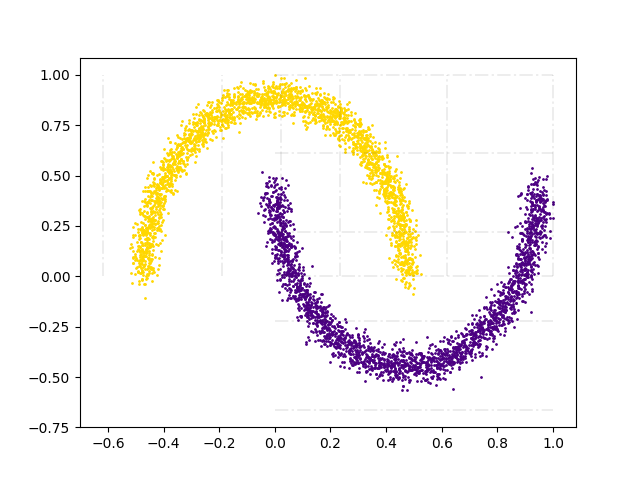
\includegraphics[width=3.5in]{img/moonsDBSCAN.png}%
\label{fig_first_case}}
\hfil
\subfloat[Clusters found by k-means.]{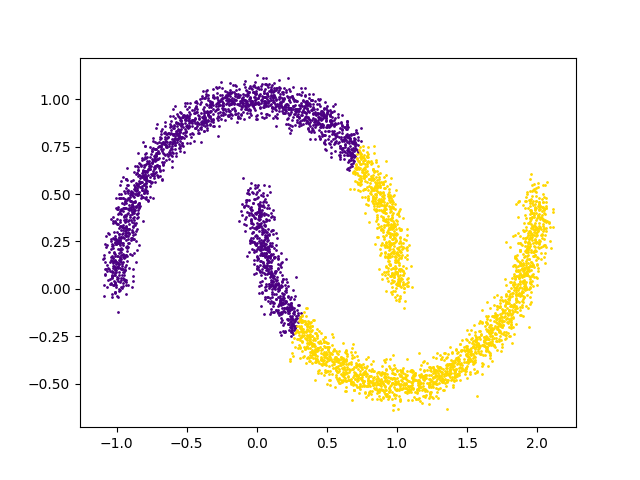
\includegraphics[width=3.5in]{img/moonsKMEANS.png}%
\label{fig_second_case}}
\caption{Comparison of the clusters provided by DBSCAN and k-means over set containing non-convex clusters.}
\label{fig_comp_clust}
\end{figure*}

\subsubsection{S.o.A for sequential and distributed implementations}

% JC: I also like this subsection. 

There are a variety of implementations of the DBSCAN raging from the more naive ones to more complex ones. As for comparison, a naive implementation following the exact guidelines of \cite{ReferencePaper} can be found \href{https://github.com/csegarragonz/DBSCAN-pyCOMPSs/blob/master/ext_versions/DBSCAN_Seq.py}{here}. One of the most extended and used versions programmed in \texttt{Python} is the one by \href{http://scikit-learn.org/stable/modules/generated/sklearn.cluster.DBSCAN.html}{Sklearn}.

When it comes to distributed implementations of the algorithm, most of them can be summarized in applying an efficient DBSCAN to a chunk of the dataset and using some sort of synchronization or MapReduce. Otherwise, the DBSCAN for PyCOMPSs reformulates the algorithm trying to adapt it to distributed architectures making sure it is still equivalent to the original implementation.

\subsection{The framework: COMPSs} \label{subec:compss_framework}

% COMPSs/PyCOMPSs definition

The \href{https://www.bsc.es/research-and-development/software-and-apps/software-list/comp-superscalar}{COMPSs} framework\cite{compss} is a programming model designed to ease the development of applications for distributed architectures. The user programs a sequential code and defines the so-called \texttt{tasks}. The COMPSs runtime infers the dependencies and schedules the executions basing on the resources available. The model is developed in Java but has bindings for both \texttt{C} and \texttt{Python}. \texttt{PyCOMPSs}\cite{pycompss} is the model chosen to develop the application. A master orchestrates a series of workes with a certain number of threads that are responsible of running tasks. In order to mark a function as a task for the scheduler to take it into account, a small decorator must be added. \texttt{COMPSs} is complemented by a set of tools for facilitating the monitoring and the post-mortem performance analysis (see Section \ref{performance}).

% \begin{figure}
% \animategraphics[autoplay,controls,loop,scale=1]{3}{img/anim-}{0.png}{4.png}
% \end{figure}

%%%%%%%%%%%%%%%%%%%%%%%%%%%%%%%%%%%%%%%%%%%%%%%%%%%%%%%%%%%%
%%%%%%%%%%%%%%%%%%%     PROPOSAL       %%%%%%%%%%%%%%%%%%%%%
%%%%%%%%%%%%%%%%%%%%%%%%%%%%%%%%%%%%%%%%%%%%%%%%%%%%%%%%%%%%

\section{Implementation Proposal} \label{sec:implementation}

% JC: Describe all implementation details of the proposal. How has DBSCAN been parallelised, parameters, etc.
% JC: Details about how it has been evaluated should be in the evaluation section.

The algorithm implemented is a reinterpretation of the one exposed in \cite{ReferencePaper}, it is still though completely equivalent. The implementation can be found in \href{https://github.com/csegarragonz/DBSCAN-pyCOMPSs}{this GitHub repository}. The main algorithm follows the structure from  Algorithm \ref{alg:main} (note that all the methods stated are later expanded and explained). It takes as an input the two required parameters: $\varepsilon$ and \texttt{min\_points} as well as the path to a distirbuted dataset stored in some sort of database\footnote{For the speciphic implementation given, the structure assumed is that of the GPFS in \ref{subsec:infrastructure} and points are assumed to be divided in a grid. Otherwise a linear classificlation should be incoporated in the pre-processing.}. It outputs the same dataset labeled with the cluster id each point belongs to.

\begin{algorithm}
  \caption{Main method for the DBSCAN algorithm. \label{alg:main}}
  \begin{algorithmic}[1]
    \Function{DBSCAN}{$data\_file$, $epsilon$, $min\_points$}
        \ForAll{$square$ \textbf{in} $data\_file$}
            \State $frag\_data \gets \text{load\_data}(data\_file)$
            \State $local\_clusters \gets \text{partial\_scan}(frag\_data)$
            \State $cluster\_map \gets \text{sync\_clusters}(local\_clusters)$
        \EndFor
        \State $frag\_data \gets \text{compss\_wait\_on}(frag\_data)$
        \State $ maps \gets \text{map\_clusters} (frag\_data, cluster\_map)$
        \ForAll{$square$ \textbf{in} $frag\_data$}
            \State $\text{expand\_clusters} (square, maps)$
        \EndFor
        \State $\textbf{return} \hspace{5pt} 1$
    \EndFunction
  \end{algorithmic}
\end{algorithm}

Note that all the methods executed within the loop statements include the \texttt{@task} decorator and therefore can potentially run in parallel. Following along, this general scheme is to be divided and each different step analysed.

\subsection{Step-by-Step analysis} \label{step_by_step}

\subsubsection{Data Loading} \label{data_pre_process}
It is important to bear in mind the punctualisation from the section above: data is assumed to be normalised (each feature of each point belonging to the interval $[0,1]$) and distributed in a file system grid-shaped. This is, if for instance the points are two-dimensional, a possible distribution would consist in the following files: \texttt{data\_0\_0.txt}, \texttt{data\_0\_1.txt}, \dots, \texttt{data\_0\_9.txt}, \texttt{data\_1\_0.txt}, \dots, \texttt{data\_9\_9.txt}. Where a point belongs to a file if each feature's first decimal position matches the file name. Were the files to be too big, two decimal places could be used as an identifier. Note that having multiples of a 100 files eases an hypothetical pre-processement if all the data was given in a single, gigantic, file.

The aim of this method is to read the data belongig to a square in our space grid, a file in the file system, and load it to memory. When doing so, each point is given a cluster id. It will be really common throughout the whole implementation to follow a recursive approach within a single task to tackle possible load imbalacments. It is such a usual practice that it is worth introducing a generic explanation.

\subsubsection*{A recursive approach to tackle load balancing} \label{recursive_approach}
The starting problem is a task that has as an input data file that can be arbitrarily big. This will cause an imbalancement in the tasks length and a decrease in the overall performance and speedup of the algorithm. It is easy to know the length of the data file and, with a simple recursive orquestrator, run tasks over chunks of the data file with a limited number of points (\texttt{THRESHOLD}). The generic structure would be that of Algorithm \ref{alg:rec-approach}. Note that \texttt{orquestrate\_task} is not a \texttt{@task} and is therefore executed by the master thread whilst \texttt{task} is indeed and will be executed by a worker.

\begin{algorithm}
  \caption{Limit the number of points processed by the same task. \label{alg:rec-approach}}
  \begin{algorithmic}[1]
    \Function{orquestrate\_task}{$data\_file, q=1, r=0$}
        \State $THRESHOLD = TH\_VALUE$
            \If{$\text{len}(data\_file)/q \geq TH\_VALUE$}
                \State $out = \text{orquestrate\_task}(data\_file, 2*q, 0)$
                \State $out = \text{orquestrate\_task}(data\_file, 2*q, 1)$
            \Else
                \State $out = \text{task}(data\_file, q, r)$
            \EndIf
        \State \textbf{return} $out$
    \EndFunction
  \end{algorithmic}
\end{algorithm}

Back to the data initialisation, for each data file, an orquestration following the structure just presented is performed upon the length of each data file with a threshold value. For each chunk then the data is loaded to a Python object and the cluster id's initially set to noise level.

\subsubsection{Partial Scan} \label{sec:partial-scan}
The aim of this method is to find core points, i.e points with over $min\_points$ neighbors and make clusters of them. For each square in our initial grid, known the grid size and $\varepsilon$, it is possible to quickly determin the number of neighbour squares necessary to correctly identify all the core points within our goal refgion. In Figure \ref{fig:neigh-loc}, it is easy to see the criterion followed. Limiting the amount of squares necessary to visit clearly reduces the computation necessary to perform the task. It is not the mos accurate space partition that can be though of but it is more simple than others and does not require any extra data structure.

\begin{figure}[!h]
\centering
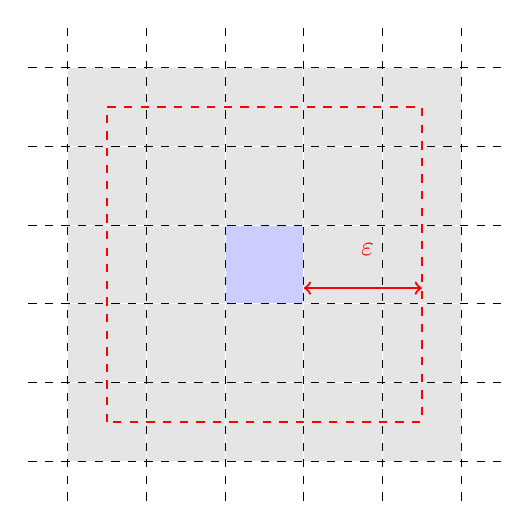
\begin{tikzpicture}[every node/.style={minimum size=1cm-\pgflinewidth, outer sep=0pt}]
    \draw[step=1cm, color=black, dashed] (-2.5,-2.5) grid (3.5,3.5);
    \node[fill=blue!20] at (0.5, 0.5) {};
    \node[fill=gray!20] at (1.5, 1.5) {};
    \node[fill=gray!20] at (2.5, 1.5) {};
    \node[fill=gray!20] at (-1.5, 1.5) {};
    \node[fill=gray!20] at (-0.5, 1.5) {};
    \node[fill=gray!20] at (0.5, 1.5) {};
    \node[fill=gray!20] at (0.5, 2.5) {};
    \node[fill=gray!20] at (0.5, -1.5) {};
    \node[fill=gray!20] at (0.5, -0.5) {};
    \node[fill=gray!20] at (-0.5, 0.5) {};
    \node[fill=gray!20] at (-1.5, 0.5) {};
    \node[fill=gray!20] at (-0.5, -0.5) {};
    \node[fill=gray!20] at (-1.5, -0.5) {};
    \node[fill=gray!20] at (-0.5, -1.5) {};
    \node[fill=gray!20] at (-1.5, -1.5) {};
    \node[fill=gray!20] at (1.5, 0.5) {};
    \node[fill=gray!20] at (2.5, 0.5) {};
    \node[fill=gray!20] at (1.5, -0.5) {};
    \node[fill=gray!20] at (2.5, -0.5) {};
    \node[fill=gray!20] at (1.5, -1.5) {};
    \node[fill=gray!20] at (2.5, -1.5) {};
    \node[fill=gray!20] at (2.5, 2.5) {};
    \node[fill=gray!20] at (1.5, 2.5) {};
    \node[fill=gray!20] at (-1.5, 2.5) {};
    \node[fill=gray!20] at (-0.5, 2.5) {};

    \draw[<->, thick, red] (1, 0.2) -- (2.5, 0.2) node[midway, above] {\vspace{-5pt} $\varepsilon$};
    \draw[thick, red, dashed] (-1.5, -1.5) rectangle (2.5, 2.5);
\end{tikzpicture}
\caption{Given the square in processment (blue) and $\varepsilon$, the squares shaded in gray will be considered neighbors. \label{fig:neigh-loc}}
\end{figure}

Once it becomes clear where possible neighbor points might be looked for, for each square in the grid, the point-limiting approach is followed. As seen in Algorithm \ref{alg:rec-approach}, the user must choose a \texttt{data-file} to divide. Inutively, and due to size constrains, one might assume that the files to be divided are the set of neighbors. In practice however, this approach proves to be mistaken. The objective of this method is to find all the core points within a square, i.e over \texttt{min\_points} neighbors. Dividing the neighbors would make impossible to decide wether a point is core or not at execution time. Given that the square being processed is also considered a neighbor itself, it is clear that there is no problem whatsoever in dividing the square to process instead of the neighbors. This explanation is exposed in Figure \ref{fig:p-scan-division}. Each worker looks for core points within their colored square and look for possible neighbors within all the gray and colored area.

\begin{figure}[!h]
\centering
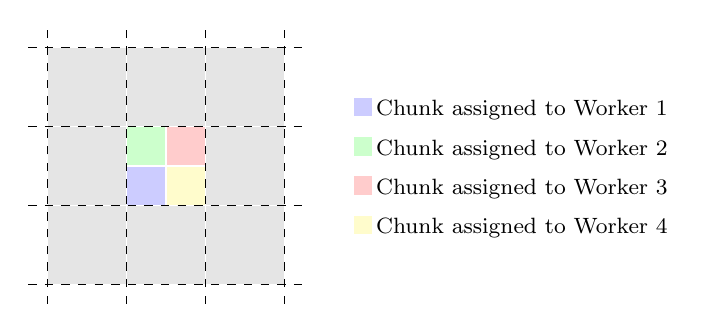
\begin{tikzpicture}[every node/.style={minimum size=1cm-\pgflinewidth, outer sep=0pt}]
    % Graphic area
    \draw[step=1cm, color=black, dashed] (-1.25,-1.25) grid (2.25,2.25);
    \node[fill=blue!20, minimum size=0.5cm-\pgflinewidth] at (0.25, 0.25) {};
    \node[fill=red!20, minimum size=0.5cm-\pgflinewidth] at (0.75, 0.75) {};
    \node[fill=green!20, minimum size=0.5cm-\pgflinewidth] at (0.25, 0.75) {};
    \node[fill=yellow!20, minimum size=0.5cm-\pgflinewidth] at (0.75, 0.25) {};
    \node[fill=gray!20] at (0.5, 1.5) {};
    \node[fill=gray!20] at (0.5, -0.5) {};
    \node[fill=gray!20] at (1.5, 1.5) {};
    \node[fill=gray!20] at (1.5, -0.5) {};
    \node[fill=gray!20] at (1.5, 0.5) {};
    \node[fill=gray!20] at (-0.5, 1.5) {};
    \node[fill=gray!20] at (-0.5, -0.5) {};
    \node[fill=gray!20] at (-0.5, 0.5) {};

    % Legend
    \node[fill=blue!20, minimum size=0.25cm-\pgflinewidth] at (3, 1.25) {};
    \node[anchor=west] at (3.05, 1.21) {\footnotesize Chunk assigned to Worker 1};
    \node[fill=green!20, minimum size=0.25cm-\pgflinewidth] at (3, 0.75) {};
    \node[anchor=west] at (3.05, 0.71) {\footnotesize Chunk assigned to Worker 2};
    \node[fill=red!20, minimum size=0.25cm-\pgflinewidth] at (3, 0.25) {};
    \node[anchor=west] at (3.05, 0.21) {\footnotesize Chunk assigned to Worker 3};
    \node[fill=yellow!20, minimum size=0.25cm-\pgflinewidth] at (3, -0.25) {};
    \node[anchor=west] at (3.05, -0.29) {\footnotesize Chunk assigned to Worker 4};

\end{tikzpicture}
\caption{Data partition for each task performing a \texttt{partial\_scan}. \label{fig:p-scan-division}}
\end{figure}

Once a task has finished scanning the area assignet to it, cluster are made out of the core points found. The output of each task is a chunk of the square dataset labeled. The labeling process is relevant and worth explaining in detail.

For each point processed, if the point is a core point then its label is updated to $-1$, if it is not a core point but has an already found core point in its neighborhood, a numerical pointer to the before mentioned core point is introduced so, in the final processing stages, labeling these reachable points will have no computing cost at all. Lastly, if it has at least more than one neighbor, the algorithm keeps track of them so that, if any gets later labeled with a cluster, it will be instant to label the first. 

Once this is finished, a reduce task is ran to combine the work performed by each worker. Since later a syncronisation task will take care of clusters that should be merged, all the clusters found by the different clusters are considered to be different and labels are updated accordingly. Note that they might need to be merged but moving this computation from the reduce task to the synchronisation one improves scalability. Algorithm \ref{alg:partial-scan} drafts this process.

\begin{algorithm}
  \caption{Looks for all the core points in a certain square and performs an initial clustering. \label{alg:partial-scan}}
  \begin{algorithmic}[1]
    \State @task()
    \Function{partial\_scan}{$sub\_square, neigh\_data$}  
        \State \Comment{Core point retrieval}
        \ForAll{$point$ \textbf{ in } $sub\_square$}
            \If{neighs($point, neigh\_data$) $\geq$ $min\_points$}
                \State $point \text{ is } core\_point $
                \Else
                \If{$core\_p \textbf{ in } \text{neighs}(point, neigh\_data)$}
                    \State $\text{link}(point, core\_point)$
                \Else
                    \State $\text{map}(point, neighs(point, neigh\_data)$
                \EndIf
            \EndIf
        \EndFor
        \State \Comment{Core point clustering}
        \State $clust\_count = 0$
        \ForAll{$point \textbf{ in } core\_points$}
            \If{$\text{close}(point,cluster)$}
                \State $point\_label = cluster\_id$
            \Else 
                \State $point\_label = clust\_count$
                \State $clust\_count += 1$
            \EndIf
        \EndFor
        \State \textbf{return} $sub\_square$
    \EndFunction
  \end{algorithmic}
\end{algorithm}

\subsubsection{Cluster Synchronization} \label{subsec:cluster_sync}
The partial scan results in each square having an arbitrary number of clusters of core points contained in them. Note that not the whole cluster must necessary be contained within the square itself but all the points contained in the cluster are core points. The following task, for each square, computes to which clusters contained in their neighbors each cluster treated can be merged with. It is worth recalling that the neighbors are those from Figure \ref{fig:neigh-loc}. As a consequence it outputs a sort of adjacency matrix where, for each cluster contained in the square, there is a list with all the contiguous clusters it can be merged with.

It is important to notice that for a cluster to be considered possible to merge with, and since all the points considered are core points, only a point from each one must be at distance under $\varepsilon$. Therefore it is possible to now apply the recursive approach not over the square data but rather over the neighbors data as presented in Figure \ref{fig:clust-sync-dp}.

\begin{figure}[!h]
\centering
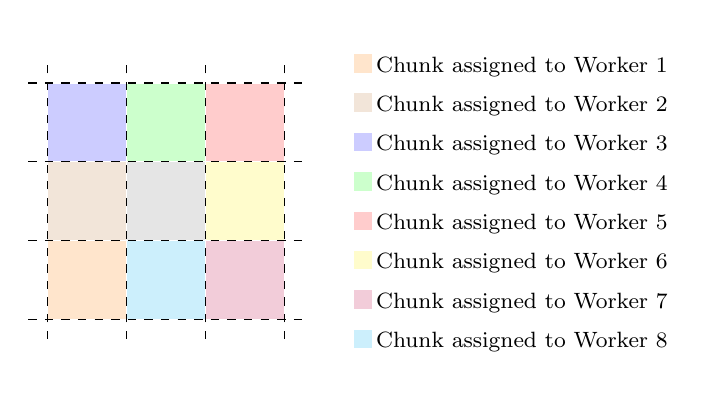
\begin{tikzpicture}[every node/.style={minimum size=1cm-\pgflinewidth, outer sep=0pt}]
    % Graphic area
    \draw[step=1cm, color=black, dashed] (-1.25,-1.25) grid (2.25,2.25);
    \node[fill=gray!20] at (0.5, 0.5) {};
    \node[fill=green!20] at (0.5, 1.5) {};
    \node[fill=cyan!20] at (0.5, -0.5) {};
    \node[fill=red!20] at (1.5, 1.5) {};
    \node[fill=purple!20] at (1.5, -0.5) {};
    \node[fill=yellow!20] at (1.5, 0.5) {};
    \node[fill=blue!20] at (-0.5, 1.5) {};
    \node[fill=orange!20] at (-0.5, -0.5) {};
    \node[fill=brown!20] at (-0.5, 0.5) {};

    % Legend
    \node[fill=orange!20, minimum size=0.25cm-\pgflinewidth] at (3, 2.25) {};
    \node[anchor=west] at (3.05, 2.21) {\footnotesize Chunk assigned to Worker 1};
    \node[fill=brown!20, minimum size=0.25cm-\pgflinewidth] at (3, 1.75) {};
    \node[anchor=west] at (3.05, 1.71) {\footnotesize Chunk assigned to Worker 2};
    \node[fill=blue!20, minimum size=0.25cm-\pgflinewidth] at (3, 1.25) {};
    \node[anchor=west] at (3.05, 1.21) {\footnotesize Chunk assigned to Worker 3};
    \node[fill=green!20, minimum size=0.25cm-\pgflinewidth] at (3, 0.75) {};
    \node[anchor=west] at (3.05, 0.71) {\footnotesize Chunk assigned to Worker 4};
    \node[fill=red!20, minimum size=0.25cm-\pgflinewidth] at (3, 0.25) {};
    \node[anchor=west] at (3.05, 0.21) {\footnotesize Chunk assigned to Worker 5};
    \node[fill=yellow!20, minimum size=0.25cm-\pgflinewidth] at (3, -0.25) {};
    \node[anchor=west] at (3.05, -0.29) {\footnotesize Chunk assigned to Worker 6};
    \node[fill=purple!20, minimum size=0.25cm-\pgflinewidth] at (3, -0.75) {};
    \node[anchor=west] at (3.05, -0.79) {\footnotesize Chunk assigned to Worker 7};
    \node[fill=cyan!20, minimum size=0.25cm-\pgflinewidth] at (3, -1.25) {};
    \node[anchor=west] at (3.05, -1.29) {\footnotesize Chunk assigned to Worker 8};

\end{tikzpicture}
\caption{Data partition for each task performing a \texttt{sync\_clusters}. \label{fig:clust-sync-dp}}
\end{figure}

To gather and synchronise all the results from the different workers it is as simple as sequentally cover all the diferent adjacency matrix found and add a cluster to the merging list if it is not there. The whole algorithm is drafted in Algorithm \ref{alg:sync-clusters}.

\begin{algorithm}
  \caption{Builds an adjacency matrix from a square w.r.t its neighbors.\label{alg:sync-clusters}}
  \begin{algorithmic}[1]
    \State @task()
    \Function{sync\_clusters}{$square, sub\_neigh\_data$}
        \State $core\_points \gets \text{get\_core\_points}(square)$
        \ForAll{$point \textbf{ in } core\_points$}
            \State $neigh\_cores \gets \text{get\_core\_points}(sub\_neigh)$
            \If{\text{close}($point, n\_point \textbf{ in } neigh\_cores$)}
                \State $adj\_matrix[point\_id].add(n\_point\_id)$
            \EndIf
        \EndFor
        \State \textbf{return} $adj\_matrix$
    \EndFunction
  \end{algorithmic}
\end{algorithm}

\subsubsection{Cluster Mapping} \label{subsec:cluster-mapping}
This is the only non-task method, i.e it must run sequentially, and it can be thought as a reduce method for each of the adjacency matrix provided by each square in the grid. This problem can be easily solved chosing the right data structure. A disjoint or union-find set immediately yields the result since it is the easier way to, given connections between nodes in a graph, find the connected components wich in this case are the real clusters.

\subsubsection{Cluster Expansion} \label{cluster_exp}
The goal of this last task is to assign a label to all the reachable points. According to Algorithm \ref{alg:partial-scan} the non-core points can either be directly pointing to another core point in which case labeling them is as simple as copying the label of the point they are looking at  or can keep track of all the points they were close to. This second case needs to be considered because, since the algorithm works sequentially point by point, it could happen that a point has a core point as a neighbor but by the time it is being porcessed the core point has not yet been processed and as a consequence he does not acknowledge it. In this case, hovering over all the points it was mapped to, and linking to the first one labeled with a cluster is sufficient. Remapping all the labels with the links found in the preceeding method is the last thing to do before printing the results to the out file. This process is drafted in Algorithm \ref{alg:expand-clusters}.

\begin{algorithm}
  \caption{Label all the reachanle points within a cluster. \label{alg:expand-clusters}}
  \begin{algorithmic}[1]
    \State @task()
    \Function{expand\_clusters}{$square\_data, mappings$}
        \State \Comment{Reachable points labeling}
        \State $non\_core\_points \gets \text{get\_non\_core}(square\_data)$
        \ForAll{$point \textbf{in} non\_core$}
            \If{$point\_id \text{ points to } core\_point$}
                \State $point\_id \gets core\_point\_id$
            \ElsIf{$point\_id \text{ maps to } core\_point$}
                \State $point\_id \gets core\_point\_id$
            \EndIf
        \EndFor
        \State \Comment{Remap the cluster labels according to the sync}
        \State $square\_data\_id \gets \text{remap}(square\_data\_id, mappings)$
        \State \text{save\_to\_file}$(square\_data)$
    \EndFunction
  \end{algorithmic}
\end{algorithm}

%%%%%%%%%%%%%%%%%%%%%%%%%%%%%%%%%%%%%%%%%%%%%%%%%%%%%%%%%%%%
%%%%%%%%%%%%%%%%%%     EVALUATION       %%%%%%%%%%%%%%%%%%%%
%%%%%%%%%%%%%%%%%%%%%%%%%%%%%%%%%%%%%%%%%%%%%%%%%%%%%%%%%%%%

\section{Evaluation} \label{sec:performance}

% JC: Add a section entry phrase for the evaluation. DONE
% JC: Subsection with the infrastructure (hardware description, software versions, etc.) DONE
% JC: Subsection with the configurations evaluated, as well as the metrics considered for the evaluation.
% JC: Results and explanations of them. If more of one evaluation is performed, divide them into subsections (e.g. performance achieved, scalability experiments, etc.) DONE

This section covers the evaluation of the implementation presented. The first subsection \ref{subsec:infrastructure} covers how was the algorithm implemented and tested. The second subsection \ref{subsec:metrics} gathers all the data collected from the different experiments performed. The last subsection \ref{subsec:critical} provides a critical review on the results, what was expected and what has been achieved.

\subsection{Infrastructure} \label{subsec:infrastructure}

As mentioned before, the algorithm has been implemented fully in Python within the PyCOMPSs framework. COMPSs version is the 2.1 and Python's is the 2.7.13 since COMPSs does not support Python 3.X. To run the program hence, the user must have COMPSs installed, the corresponding Python version and the numeric python library (numpy). The algorithm can be ran both locally and in a cluster, in the project's GitHub repository there is a shell script (\texttt{run.sh}) that contains methods to invoke the DBSCAN both as local host (through \texttt{runcompss} command) and to a queuing system (through \texttt{enqueue\_compss} command). 

The experiments were ran on a cluster located in Barcelona. The \href{https://www.bsc.es/user-support/mn4.php#systemoverview}{Mare Nostrum 4} (MN4) is the fourth generetion of supercomputers located in the \href{https://www.bsc.es}{Barcelona Supercomputing Center - Centro Nacional de Supercomputacion (BSC-CNS)} its current Linpack Rmax Performance is 6.2272 Petaflops and it has been running since early July 2017. It is equipped with 48 racks with 3456 nodes. Each node has two Intel Xeon Platinum chips with 24 processors per unit. COMPSs through its queuing script for clusters, \texttt{enqueue\_compss}, requires each node on exclusivity. Therefore from now on, whenever a node is mentioned it must be considered that no other program is going to be running there besides our execution. Additionally the queuing script incorporates a \texttt{cpus\_per\_node} flag that determines the number of processors running in each node.

\subsection{Runtime Metrics} \label{subsec:metrics}

To evaluate the algorithm's performance for different dataset sizes (all three dimensional but with different number of points) the execution time has been measured. This duration is computed inside the python method using the built-in tools and printed through the standard output. For the same dataset, a batch of executions with different number of workers was performed to test the algorithm's scalability. The input parameters vary between different data sizes but never inside the same batch. All the executions were ran in MN4 (\ref{the_machine}) with Scratch file system. Results are summarized in Table \ref{performance_table}

\begin{table*}[!t]
\centering
\caption{Performance measured on MN4 without tracing and 16 CPUs per node.}
\label{performance_table}
\begin{tabular*}{\textwidth}{c|cc|cc|cc|cc|cc}
 \textbf{SCRATCH}   & \textbf{NP=16} & \textbf{10k} & \textbf{NP = 16} & \textbf{20k} & \textbf{NP = 32} & \textbf{50k} & \textbf{NP = 32} & \textbf{100k} &  \textbf{NP=32} & \textbf{ 200k}\\ \cline{2-11} 
\textbf{Workers}     & \textbf{Time (sec)}   & \textbf{SUp}   & \textbf{Time (sec)}     & \textbf{SUp}   & \textbf{Time (sec)}     & \textbf{SUp}   & \textbf{Time (sec)}    & \textbf{SUp}    & \textbf{Time (sec)}   & \textbf{SUp} \\ \cline{1-11}
\textbf{1}           & 36.12        & 1.00              & 125.03          & 1.00              & 820.14           & 1.00              & 3160.46          & 1.00  &   15030.99 & 1.00          \\
\textbf{2}           & 22.47          & 1.63           & 71.66            & 1.74           & 423.36           & 1.93           & 1623.92          & 1.94 & 7659.83 & 1.96        \\
\textbf{3}           & 18.05          & 2.02           & 55.04           & 2.27           & 308.014          & 2.62           & 1165.10         & 2.71 & 4547.23 & 3.3           \\
\textbf{4}           & 15.91         & 2.25           & 45.60           & 2.74           & 249.59           & 3.28           & 910.30            & 3.47   & 3634.97 & 4.13        \\
\textbf{5}           & 15.01          & 2.40           & 42.49           & 2.94           & 227.93           & 3.59           & 777.19          & 4.06  & 3134.47 & 4.79         \\
\textbf{6}           & 14.55          & 2.48           & 40.23            & 3.16           & 196.69           & 4.16           & 703.90            & 4.48 & 2736.65 & 5.49           \\
\textbf{7}           & 14.3           & 2.52           & 36.36           & 3.43           & 184.00              & 4.45           & 620.53          & 5.09 & 2557.32 & 5.87           \\
\textbf{8}           & 13.64         & 2.64           & 33.61           & 3.72           & 171.00              & 4.79           & 609.21          & 5.18 & 2376.56 & 6.32           \\
\textbf{16}          & 13.45          & 2.68           & 29.02           & 4.30           & 143.00              & 5.73           & 433.12          & 7.29 & 1565.82 & 9.59           \\ \cline{1-11}
\textbf{Seq} & 4690.80         &                & ---              &                & ---              &                & ---              & & --- &                
\end{tabular*}
\end{table*}

\begin{figure}[h!]
\centering	
\begin{tikzpicture}
\begin{axis}[
height=2in,
width=3.5in,
    scaled x ticks = false,
    xlabel = {\# Workers},
    grid = major,
    ylabel = {Speed Up},
    legend entries={10k, 20k, 50k, 100k, 200k}, legend style={at={(0.05,-0.25)},anchor=north west, draw=none, legend columns=-1}
    %xtick={0.028503, 0.0427553,0.0570},
    %xticklabels={$l-2\lambda$, $l-\lambda$,$l$},
    %ytick={0,1,2},
    %yticklabels={0,$|E_{0i}|$,$2|E_{0i}|$},
]
\addplot[mark=o, thick, blue] table {data/10k.dat};
\addplot[mark=o, thick, orange] table {data/20k.dat};
\addplot[mark=o, thick, red] table {data/50k.dat};
\addplot[mark=o, thick, green] table {data/100k.dat};
\addplot[mark=o, thick, purple] table {data/200k.dat};
%Here the blue parabloa is defined
\end{axis}
\end{tikzpicture}
\caption{Speed Up as a function of the number of workers for different datasets.}
\label{speed_up}
\end{figure}

In figure \ref{speed_up} there is a speed up vs number of workers plot. To understand why it increases as the number of points increases check section \ref{q_coi_passa}. Additionally, a runtime vs number of workers plot can be found at \ref{rt_plot}.

\begin{figure}[h!]
\centering	
\begin{tikzpicture}
\begin{axis}[
height=2in,
width=3.5in,
    scaled x ticks = false,
    xlabel = {\# Workers},
    grid = major,
    ylabel = {Execution Time (sec)},
    legend entries={10k, 20k, 50k, 100k, 200k}, legend style={at={(0.05,-0.25)},anchor=north west, draw=none, legend columns=-1}
    %xtick={0.028503, 0.0427553,0.0570},
    %xticklabels={$l-2\lambda$, $l-\lambda$,$l$},
    %ytick={0,1,2},
    %yticklabels={0,$|E_{0i}|$,$2|E_{0i}|$},
]
\addplot[mark=o, thick, blue] table {data/10kRT.dat};
\addplot[mark=o, thick, orange] table {data/20kRT.dat};
\addplot[mark=o, thick, red] table {data/50kRT.dat};
\addplot[mark=o, thick, green] table {data/100kRT.dat};
\addplot[mark=o, thick, purple] table {data/200kRT.dat};
%Here the blue parabloa is defined
\end{axis}
\end{tikzpicture}
\caption{Execution time as a function of the number of workers for different datasets.}
\label{rt_plot}
\end{figure}

\subsection{Critical Analysis} \label{subsec:critical}

\subsubsection{Dependence on the scale parameters:}

From the explanation in Section \ref{the_algorithm} it is easy to see that the paradigm has shifted from a two parameter algorithm to a four one. In the one hand this enables, when run by someone familiar to it, the algorithm to adapt better to mutable resources and data loads. In the other hand this also increases the variability of the performance, may be a drawback at some points and makes the implementation not 100\% structure-unaware.

Emphasizing on this two extra parameters, one of them has not got a clear impact on the runtime metrics. The number of comparisons executed by a worker, \texttt{numComp} will determine a certain type of task's length but won't increase their variability. However, \texttt{numParts} chunks the data again having a direct effect on the number of clusters initially found and consequently on the number of tasks performed at the syncing stage. In addition to that, it reduces the average task duration and at the same time makes tasks less homogeneous. This process causes bigger executions' (more points and assigned nodes) behavior more volatile. In spite of that, this scale parameter is necessary to ensure the algorithm's scalability, otherwise it would depend entirely on the data distribution.

\begin{figure}[!h]
\centering
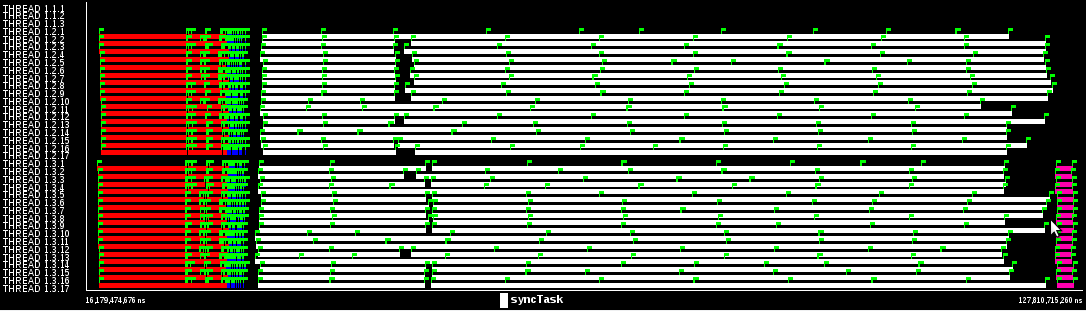
\includegraphics[width=3.5in]{img/traca_compacte.png}
\caption{Tracing with 10k points and $\texttt{numParts}=16$.}
\label{traca_bona}
\end{figure}

To dig in this sections where the algorithm is not performing as expected, or at least not as desired, we undergo a performance analysis using tracing (\href{https://tools.bsc.es/paraver}{Paraver}). In Figure \ref{traca_bona} there is an example of a small execution with  $\texttt{numParts}=16$ (relatively small value of the parameter) and 10000 points. Consequently with the above lines a homogeneous trace is obtained. In Figure \ref{traca_caca} the opposite behavior is exposed. For this second execution the number of points was around 20000 and $\texttt{numParts}=32$. It is easy to see that tasks durations become much more unstable (green flags indicate a task's beginning and ending) and they are not so easily scheduled by the COMPSs runtime.

\begin{figure}[!h]
\centering
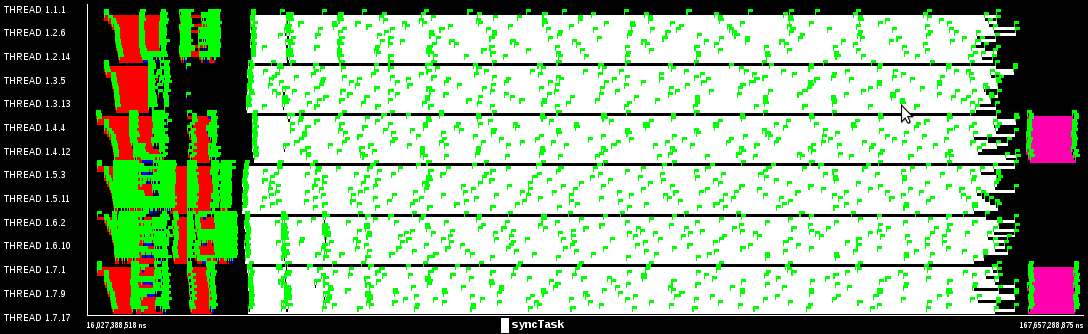
\includegraphics[width=3.5in]{img/traca_mes_caca.png}
\caption{Tracing with 20k points and $\texttt{numParts}=32$.}
\label{traca_caca}
\end{figure}

\subsubsection{On memory, CPUs per node and scalability:} \label{q_coi_passa}

Another issue faced when testing the algorithm is the memory vs cpu per node paradigm. Initially each node has 2GB of RAM, however if the user requests less CPUs per node and exclusivity each worker will virtually have more random access memory since the whole batch is divided between the running threads. When the dataset tends to get bigger and bigger, the memory requested increases as well. Hence the performance at some points might be better with less \texttt{cpus\_per\_node} in spite of the time lost with inter-node communication. To dig deeper into this situation, another set of tests is performed. Results are summarized in Table \ref{cpusComparison}. The \texttt{cpus\_per\_node} values to be compared are 16 and 48. 48 is 16 times 3, therefore to perform a fair comparison the number of workers assigned to the 16 \texttt{cpus\_per\_node} test must be three times the ones assigned to the 48 \texttt{cpus\_per\_node} one. Surprisingly enough given the reasoning above, results do not show a clear dominance of 16 CPUs per node tests over 48 CPUs ones with small datasets. As the size of the input grows and as more calculations are required, the performance is the predicted and 16 \texttt{cpus\_per\_node} tests are quicker.

\subsubsection{On time complexity}

Figures \ref{timeComplexity1} and \ref{timeComplexity2} plot the evolution of the execution time as a function of the size of the input, i.e the number of points, for a fixed number of working nodes and two different \texttt{cpus\_per\_node} parameters, 16 and 48 respectively. \ref{q_coi_passa} shows that there is no evident difference between the two options, as a consequence both Figures look really similar. The main conclusion one can deduce is that, the higher the number of workers (or CPUs in general) the least the application behaves quadratically as its naive sequential implementation and the better PyCOMPSs performs.

\subsubsection{Testing with real data and comparing with S.o.A implementations}

All the previous tests have been performed with synthetic data. The application must as well prove to be useful in real-life applications and when compared to other implementations. A real case use is the one presented in \cite{toolsDBSCAN} where clustering is applied to an app trace to "outline the different trends of the CPU computation areas of parallel applications". Within the same paper, an implementation of the DBSCAN is proposed and thus we will be able to compare both performances. The trace used is one corresponding to:

%%%%%%%%%%%%%%%%%%%%%%%%%%%%%%%%%%%%%%%%%%%%%%%%%%%%%%%%%%%%
%%%%%%%%%%%%%%%%%       CONCLUSIONS     %%%%%%%%%%%%%%%%%%%%
%%%%%%%%%%%%%%%%%%%%%%%%%%%%%%%%%%%%%%%%%%%%%%%%%%%%%%%%%%%%


\section{Conclusion} \label{sec:conclusion}

% Conclusions structure:
% - Describe the achievements of the work (DBSCAN parallelization, performance results, etc.)
% - Considerations (if any).
% - Future work.
%
% JC: There shouldn't be tables of results nor graphs in this section. They should be in the evaluation section.
% JC: I wouldn't divide it in subsections.

Following along the reasoning from \ref{subsec:critical}, the algorithm is really sensitive to changes in the input parameters. Thus this parameters should somehow depend on the resources available, however that would make the algorithm not structure-unaware. This might be one of the reasons why scalability and speed up is not exactly as desired since all the tests for the same dataset are performed under the same input parameters (to be able to compare them). Therefore the measured speedup might be worse in comparison to if we were to run the algorithm manually test by test. 

\begin{table*}[!h]
\centering
\caption{Execution time comparison with the same number of CPUs but different number of workers and different CPUs per node. Time measured in seconds.}
\label{cpusComparison}
\begin{tabular*}{.95\textwidth}{c|cc|cc|cc|cc|cc}
\textbf{Comparison CPUS per Node} & \multicolumn{2}{c|}{\textbf{10k}} & \multicolumn{2}{c|}{\textbf{20k}} & \multicolumn{2}{c|}{\textbf{50k}} & \multicolumn{2}{c|}{\textbf{100k}} &
\multicolumn{2}{c}{\textbf{200k}}
\\ \hline
\textbf{\#Workers - 16 (48)}      & \textbf{16}     & \textbf{48}     & \textbf{16}     & \textbf{48}     & \textbf{16}     & \textbf{48}     & \textbf{16}      & \textbf{48}   & \textbf{16}     & \textbf{48}  \\ \hline
\textbf{3 (1)}                    & 23.44           & 21.81           & 68.22           & 63.6            & 375.47          & 366.49          & 1326.732         & 1322.73  & 5308.99 & 5501.241035    \\
\textbf{6 (2)}                    & 16.74           & 16.94           & 46.15           & 44.62           & 233.71          & 230.68          & 790.97           & 785.68   & 3205.49 & 3412.54       \\
\textbf{9 (3)}                    & 16.609          & 16.42           & 39.71           & 37.77           & 190.39          & 186.69          & 623.78           & 627.52   & 2427.87 & 2451.26       \\
\textbf{12 (4)}                   & 17.78           & 15.74           & 34.43           & 36.01           & 167.83          & 173.65          & 555.06           & 544.66    & 2039.61 & 2012.89      \\
\textbf{15 (5)}                   & 17.23           & 16.92           & 33.71           & 33.177          & 163.87          & 158.08          & 487.01           & 480.03     & 1707.57 & 1842.83     \\
\textbf{18 (6)}                   & 16.76           & 15.63           & 33.166          & 33.84           & 156.11          & 149.75          & 461.73           & 446.91   & 1486.20 & 1708.76      
\end{tabular*}
\end{table*}

\begin{figure}[t]
\centering
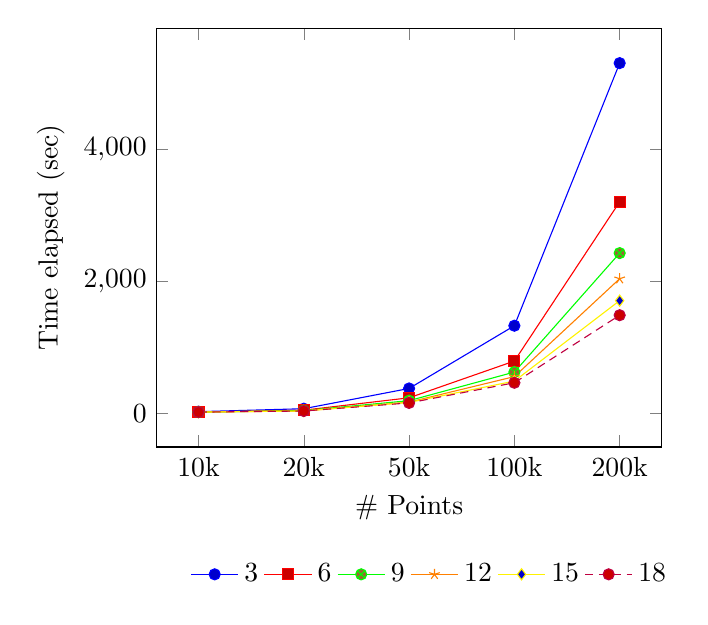
\begin{tikzpicture}
    \begin{axis}
        [
        ,width=8cm
        ,xlabel=\# Points
        ,ylabel=Time elapsed (sec)
        ,xtick=data,
       %,xtick={0,1,...,3}
        ,xticklabels={10k,20k,50k,100k, 200k}
        ,legend entries={3, 6, 9, 12, 15, 18}, legend style={at={(0.05,-0.25)},anchor=north west, draw=none, legend columns=-1}
        ]
        \addplot+[sharp plot] coordinates
        {(0,23.44) (1,68.22) (2,375.47) (3,1326.73) (4, 5308.99)};
        \addplot+[sharp plot, red] coordinates
        {(0,16.74) (1,46.15) (2,233.71) (3,790.97) (4, 3205.49)};
        \addplot+[sharp plot, green] coordinates
        {(0,16.609) (1,39.71) (2,190.39) (3,623.78) (4, 2427.87)};
        \addplot+[sharp plot, orange] coordinates
        {(0,17.78) (1,34.43) (2,167.83) (3,555.06) (4, 2039.61)};
        \addplot+[sharp plot, yellow] coordinates
        {(0,17.23) (1,33.43) (2,163.87) (3,487.01) (4, 1707.57)};
        \addplot+[sharp plot, purple] coordinates
        {(0,16.76) (1,33.16) (2,156.11) (3, 461.73) (4, 1486.2)};
    \end{axis}
\end{tikzpicture}
\caption{Evolution of time elapsed with a fixed number of workers. 16 CPUs per node. \label{timeComplexity1}}
\end{figure}

\begin{figure}[t]
\centering
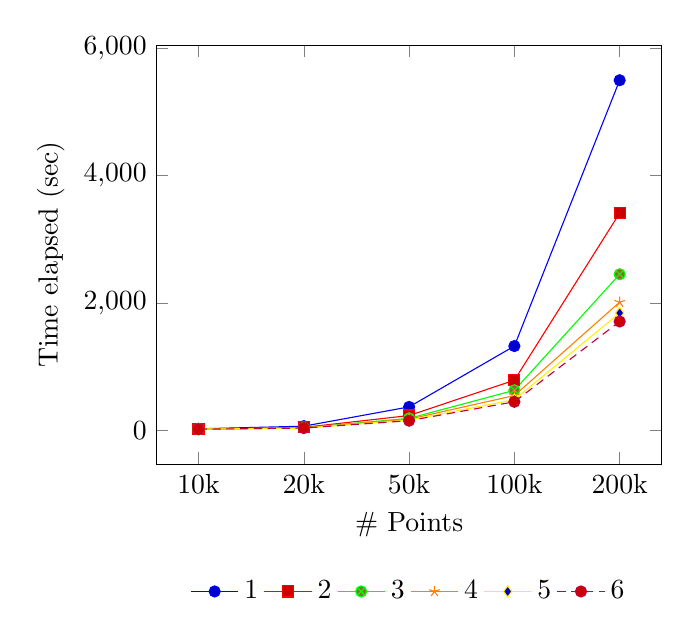
\begin{tikzpicture}
    \begin{axis}
        [
        ,width=8cm
        ,xlabel=\# Points
        ,ylabel=Time elapsed (sec)
        ,xtick=data,
       %,xtick={0,1,...,3}
        ,xticklabels={10k,20k,50k,100k, 200k}
        ,legend entries={1, 2, 3, 4, 5, 6}, legend style={at={(0.05,-0.25)},anchor=north west, draw=none, legend columns=-1}
        ]
        \addplot+[sharp plot] coordinates
        {(0,21.81) (1,63.6) (2,366.49) (3,1322.73) (4, 5501.24)};
        \addplot+[sharp plot, red] coordinates
        {(0,16.94) (1,44.62) (2,230.68) (3,785.68) (4, 3412.54)};
        \addplot+[sharp plot, green] coordinates
        {(0,16.42) (1,37.77) (2,186.69) (3,627.52) (4, 2451.26)};
        \addplot+[sharp plot, orange] coordinates
        {(0,15.74) (1,36.01) (2,173.83) (3,544.66) (4, 2012.89)};
        \addplot+[sharp plot, yellow] coordinates
        {(0,16.92) (1,33.17) (2,158.08) (3,480.03) (4, 1842.83)};
        \addplot+[sharp plot, purple] coordinates
        {(0,15.63) (1,33.84) (2,149.75) (3, 446.91) (4, 1708.76) };
    \end{axis}
\end{tikzpicture}
\caption{Evolution of time elapsed with a fixed number of workers. 48 CPUs per node.} \label{timeComplexity2}
\end{figure}

\subsection{Further Development and Improvement Proposals} \label{further_development}
The main development recommended would be performing a smart guess at execution time of the scale parameters. Empirically it has been proven that if the user is able to choose the right parameters, the algorithm is going to have a great performance. As a consequence, being able to guess them at execution time would guarantee a stability that for this moment can not be ensured.

Secondly, the DBSCAN method could be expanded to a generalized DBSCAN to detect arbitrary cluster densities removing the dependencies to the input parameters, \texttt{minPoints} and $\varepsilon$.

Lastly and in the opposite direction of the second proposal, some research into parallel optimization models so to guess the input parameters (rather than using a thumb rule) could be done.

%%%%%%%%%%%%%%%%%%%%%%%%%%%%%%%%%%%%%%%%%%%%%%%%%%%%%%%%%%%%
%%%%%%%%%%%%%%       ACKNOWLEDGEMENTS     %%%%%%%%%%%%%%%%%%
%%%%%%%%%%%%%%%%%%%%%%%%%%%%%%%%%%%%%%%%%%%%%%%%%%%%%%%%%%%%


\section*{Acknowledgements}

Acks

% JC: In this section we will include the acknowledgements required. Don't worry about it by now. It will be just a paragraph with some references to projects and funding.

%%%%%%%%%%%%%%%%%%%%%%%%%%%%%%%%%%%%%%%%%%%%%%%%%%%%%%%%%%%%
%%%%%%%%%%%%%%%%%       BIBLIOGRAPHY     %%%%%%%%%%%%%%%%%%%
%%%%%%%%%%%%%%%%%%%%%%%%%%%%%%%%%%%%%%%%%%%%%%%%%%%%%%%%%%%%


\begin{thebibliography}{1}
\bibitem{compss}
Badia, R. M., J. Conejero, C. Diaz, J. Ejarque, D. Lezzi, F. Lordan, C. Ramon-Cortes, and R. Sirvent \textit{COMP Superscalar, an interoperable programming framework} SoftwareX, Volumes 3–4, December 2015, Pages 32–36, 
\bibitem{related_1}
D. Arlia and M. Coppola, \textit{Experiments in Parallel Clustering
with DBSCAN} in Euro-Par 2001, Springer, LNCS, 2001, pp.
326-331.
\bibitem{related_2}
 S. Brecheisen et al., \textit{Parallel Density-Based Clustering of Complex Objects} Advances in Knowledge Discovery and
Data Mining, pp. 179-188, 2006.
\bibitem{related_3}
Yaobin He et al. \textit{MR-DBSCAN: a scalable MapReduce-based DBSCAN algorithm for heavily skewed data} Frontiers of Computer Science, vol 8, no. 1, pp 83-99, 2014.
\bibitem{related_4}
Md. Mostofa Ali Patwary et al. \textit{A new scalable parallel DBSCAN algorithm using the disjoint-set data structure} Conference: High Performance Computing, Networking, Storage and Analysis (SC), 2012 
\bibitem{related_5}
Alessandro Lulli, Matteo Dell'Amico, Pietro Michiardi, Laura Ricci \textit{NG-DBSCAN: scalable density-based clustering for arbitrary data}. Proceedings of the VLDB Endowment Volume 10 Issue 3, November 2016, p. 157-168 
\bibitem{ReferencePaper}
Ester, Martin Kriegel, Hans-Peter Sander, Jorg Xu, Xiaowei (1996). \textit{A density-based algorithm for discovering clusters in large spatial databases with noise.} Proceedings of the Second International Conference on Knowledge Discovery and Data Mining (KDD-96)
\bibitem{kmeans}
MacQueen, J. B. (1967). \textit{Some Methods for classification and Analysis of Multivariate Observations.} Proceedings of 5th Berkeley Symposium on Mathematical Statistics and Probability.
\bibitem{pycompss}
Enric Tejedor, Yolanda Becerra, Guillem Alomar, Anna Queralt, Rosa M. Badia, Jordi Torres, Toni Cortes, Jesús Labarta, \textit{PyCOMPSs: Parallel computational workflows in Python}  IJHPCA 31(1): 66-82 (2017)
\bibitem{toolsDBSCAN}
J. Gonzalez, J. Gimenez, J. Labarta. \textit{Automatic detection of parallel applications computation phases}.
\end{thebibliography}


\end{document}


